%*****************************************
\chapter{Spatial back-mapping of single cell RNA-seq data}\label{ch:mapping}
%*****************************************

\section{Single cell RNA sequencing, building a map of the full transcriptome}\label{sec:single_cell_rnaseq}
  \subsection{Single cell RNA sequencing}
	The scale shift from tissue to single cell is harder to achieve for RNA-seq than for in-situ hybridization assays. As described in the Introduction \ref{sec:gene_expression_lab}, an important factor for the success of RNA-seq assays is the input quantity of RNA to be sequenced. Taking mammalian cells as a reference, the quantity of RNA depends a lot on the cell type considered and can vary between 10 and 50 pg per cell, only 2\% of which is mRNA \citep{iscove02,islam11}. With such a small input quantity, distinguishing biological variation between different cells from the technical variation linked to mRNA capture rates and to cDNA amplification protocols is extremely challenging.\\

	However, with the creation of new protocols \citep{ramskold12,tang09}, and the rise of microfluidics approaches that faciliate the extraction and sequencing of single cells \citep{ozsolak10}, the last couple of years have seen a dramatic increase in the number of single cell RNA-seq based studies \citep{islam13,marinov13,yan13,staahlberg13,deng14}. However, challenges still need to be overcome in order to analyse further complex tissues using such approaches.
	
  \subsection{Technical noise in single cell RNA-seq data}
  Single cell RNA-seq is also prone to high levels of noise. This technical noise is caused by the minute amounts of starting RNA material. A study led by Philip Brennecke, Simon Anders and Jong Kyoung Kim \citep{brennecke13}, proposes a statistical method to overcome this high noise level and distinguish between biological variation and technical variation in the gene expression levels.\\
  
  To illustrate the dramatic increase in noise level, they used a series of dilution assays, reducing step by step (5000 pg, 500 pg, 50 pg, 10 pg) the input quantity of RNA fragments extracted from total \species{Arabidobsis thaliana} RNA with two technical replicates each time using the single cell RNA-seq Tang protocol \citep{tang09}. The authors of the study let me analyse this data, and after normalizing by the size factor using the Bioconductor package DESeq \citep{anders10} the scatter plots shown in Figure \ref{fig:dilutions} were generated. \\
  
  It is clear from these dilution assays that the noise level is correlated with the input quantity. Even though highly expressed genes are consistently well quantified even with 10 pg input material, for most of the genes, with less than 50 pg input RNA it seems dangerous to assume the results of single cell RNA-seq as quantitative with the current technological capabilities.
  
\begin{figure}[h]
        \myfloatalign
        \subfloat[5000 pg input RNA.]
        {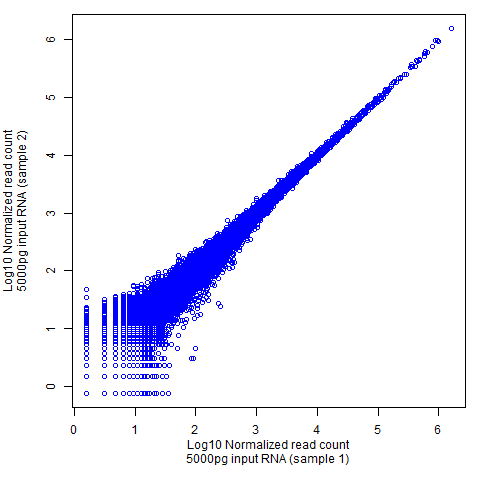
\includegraphics[width=.45\linewidth]{gfx/chapter2/5000pg.png}} \quad
        \subfloat[500 pg input RNA.]
        {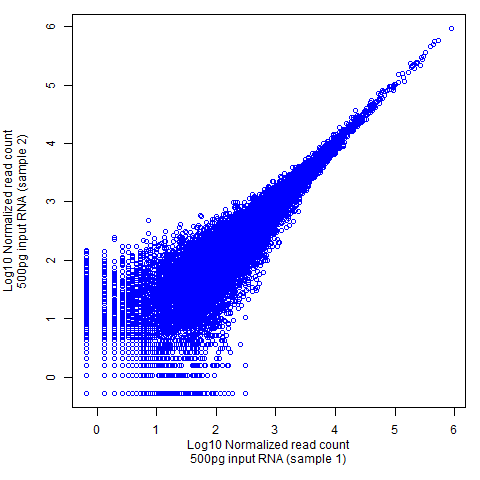
\includegraphics[width=.45\linewidth]{gfx/chapter2/500pg.png}} \\
        \subfloat[50 pg input RNA.]
        {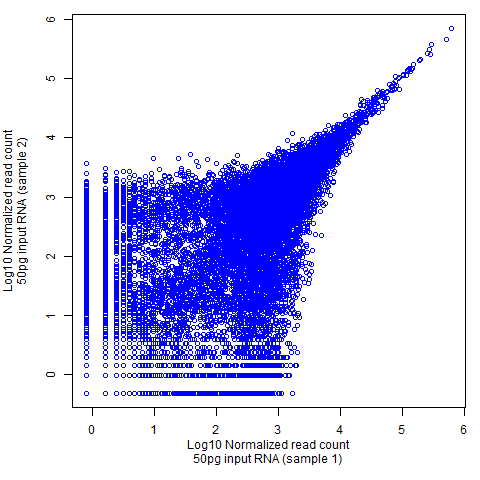
\includegraphics[width=.45\linewidth]{gfx/chapter2/50pg.png}} \quad
        \subfloat[10 pg input RNA.]
        {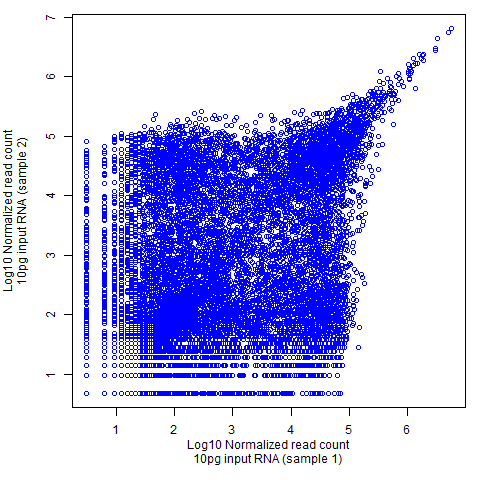
\includegraphics[width=.45\linewidth]{gfx/chapter2/10pg.png}}
        \caption{Dilution series of total A. thaliana RNA}\label{fig:dilutions}
\end{figure}


	The paragraphs above have shown that neither in-situ hybridization nor RNA-seq data are fully quantitative when the scale is lowered to the single cell level. To avoid problems linked to the noise level in the rest of this study, a solution was to binarize single cell datasets. However, binarization is not a trivial problem as discussed in the following section.

  \subsection{Mapping back gene expression to a spatial reference}

	Single cell RNA-seq captures a snapshot of the entire transcriptome of a given cell at a given point in time. However, to analyse cells from a complex tissue, current protocols require that the tissue be reduced to a suspension of single independent cells. This prevents the user from keeping track of any spatial information about the cells. Hence, when analysing single cell RNA-seq data from a complex tissue, back-mapping every cell to its original location becomes a crucial problem.\\ 
	
	A recent paper published in Cell \citep{durruthy14} describes a purely mathematical way to approximate the spatial organisation of sequenced single cells using a series of statistical methods to segregate and map single cells RNA-seq data obtained from mice otocysts onto a reference sphere. The method mainly based on Principal Components Analysis, allows them to reconstruct a ``image'' of the otocyst.\\
	
	To push the method presented in \citep{durruthy14} further, we could achieve back-mapping of the single cells to a different dataset with a spatial reference. This reference should consist of an independent assay where gene expression in the considered tissue is defined for enough genes at a spatially small enough resolution to find for each sequenced cell, if not its exact original location, at least a restricted region of the tissue from which the sequenced cell originated with a high probability.\\
	
	Fortunately, in-situ hybridization assays provide exactly this type of data and I will present in the last section of this Chapter (\ref{sec:back_mapping_platy}) a methodological proof-of-concept of this back-mapping in the brain of \platy{} with 72 sequenced single cells. However, before that, I will discuss the impact of the noise level in both in-situ hybridization and single cell RNA-seq assays on the quantitative nature of the resulting datasets.
	
\section{Preliminary results on single cell RNA-seq in \platy{}'s brain}\label{sec:back_mapping_platy}
  \subsection{Single cell RNA-seq in Platynereis' brain}
  
    	A collaborations with Kaia Achim in the Arendt lab in EMBL provided us with a unique RNA-seq dataset of 72 single cells from \platy{}'s 48hpf developing brain. 
    	
	Experimentally, the work consisted in setting up \platy{} batches, picking up 50-100 individuals at 48hpf. These were washed in Ca-Mg free sea water and incubated in a mixture of pronase which breaks extracellular matrix and thioglycolate (helps to break the chorion). After this treatment, the trunks and epispheres (brains) were separated. 40-60 epispheres were then picked out, transferred to Phosphate buffered saline (PBS) and then incubated for 1 minute in PBS containing collagenase to break more extracellular matrix. After two PBS washes, the cells were dissociated by pipetting up and down then washed again in 1 ml of PBS and concentrated by centrifuging (1 min, 1000 rpm). Cells were re-suspended in 20 microliters of PBS, of which 5 microliters could be loaded on the capture chip.\\

	Fluidigm's C1 Single-Cell Auto Prep System instrument with the Fluidigm Single-Cell Auto Prep IFC chip optimized for 10-17 micron cells were used as shown in Figure \ref{fig:singlecell_chip}. The reverse transcription was performed using Clontech SMARTer Ultra Low Input RNA Kit and for on-chip PCR the Clontech ADVANTAGE-2 PCR kit. Sequencing libraries were prepared using Nextera DNA Sample Preparation kit from Illumina.\\
	
\begin{figure}[h]
        \myfloatalign
        \subfloat[Fluidigm C1 chip with 96 wells. Image taken from Fluidigm website]
        {\label{fig:c1}
        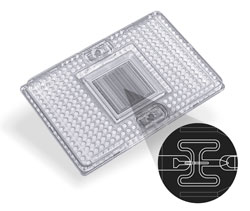
\includegraphics[width=.45\linewidth]{gfx/chapter2/c1.jpg}} \quad
        \subfloat[One cell from \platy{}'s brain captured in the chip (circled in red). Image generated by Kaia Achim]
        {\label{fig:chip}%
         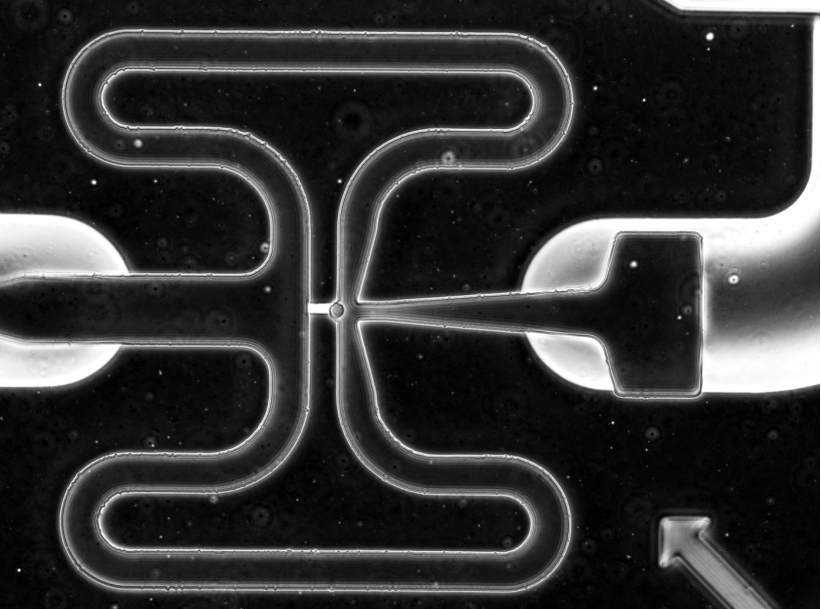
\includegraphics[width=.45\linewidth]{gfx/chapter2/chip.png}}
        \caption{Microfluidics single cell sequencing with C1 chips.}\label{fig:singlecell_chip}
\end{figure}
	

	With two chips and a capture rate of 65\%, 72 libraries were sequenced including 11 cells from first chip. From the second chip 35 live single cells, 17 dead single cells, 3 wells containing 2 cells, one with 4 cells, and 3 unsure ones resulting in 72 raw reads files as shown in Table \ref{tab:rna_seq_res}.\\	
	
\begin{table}
    \myfloatalign
  \begin{tabularx}{\textwidth}{X|c} \toprule
    Chips used & 2 \\
    Capture rate  & 65\%\\
    Libraries sequenced & 72 \\
	Live single cells & 38 \\
	Dead single cells & 15 \\
	Debris + live single cell & 4 \\
	Multiple cells & 6 \\
	Debris/unsure & 9\\
  \end{tabularx}
  \caption{Results over two C1 chips. The experiments were conducted by Kaia Achim.}\label{tab:rna_seq_res}
\end{table}
  	
	Of course those results do not include the spatial localization of the cells as the protocol requires the separation of the coherent tissue into a cell suspension. As a crucial point in any dowstream analysis, being able to map back the single cells to their original location in the brain is required. To that end, I took advantage of the spatially localized in-situ hybridization described in the previous section.\\


  \subsection{Mapping RNA-seq data back to PrimR in-situ hybridization assays}
  	Firstly, Bowtie \citep{langmead12} was used to map the RNA-seq raw reads to a reference containing the sequences of the 86 reference genes composing the in-situ hybridization data. The resulting dataset comprises the number of reads mapped back to each of the 86 genes in the 72 cells sequenced (Figure \ref{fig:backmap}).\\
  	
  	 In order to map back to the in-situ hybridization data, the chosen approach consisted of extracting the genes that were the most specifically expressed for each sequenced cell, before comparing this specific fingerprint to the in-situ 3D data in order to isolate the regions of the brain where those specific genes are co-expressed.\\
  	
	\begin{figure}[h]
\centerline{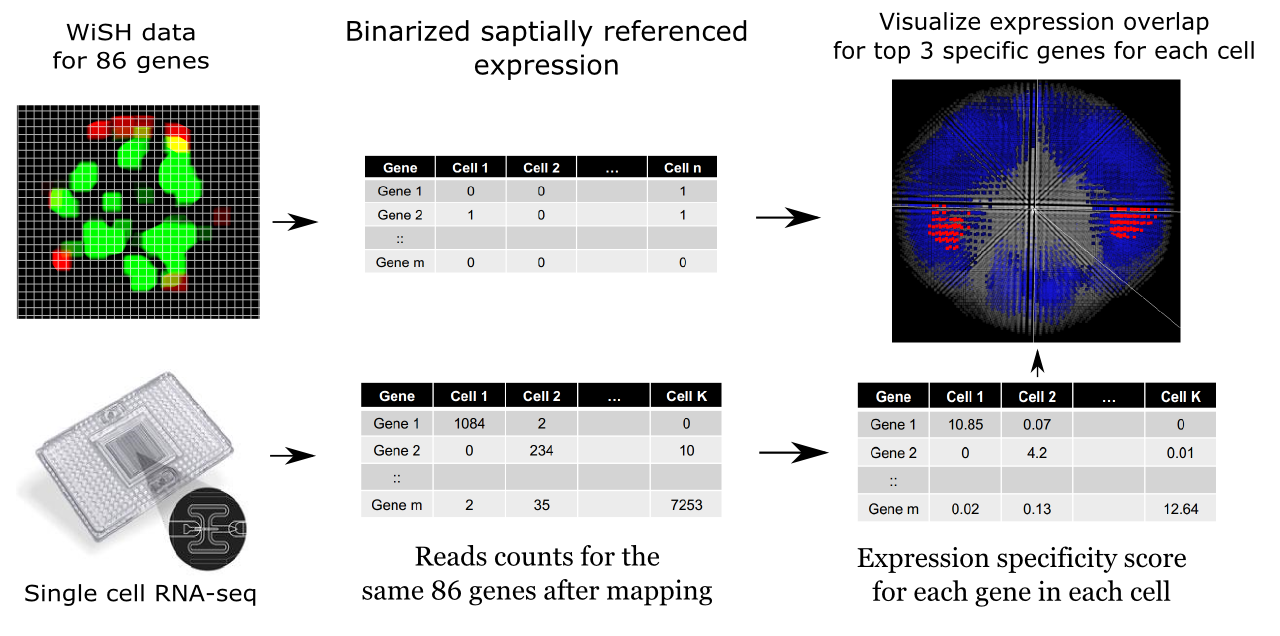
\includegraphics[width=1.5\linewidth]{gfx/chapter2/backmap.png}}
\caption{{\bf Spatial back mapping of single cell RNA-seq.} The binarized in-situ hybridization data provides the spatial reference onto which the single cell results will be mapped. All the single cells sequenced are put together and a expression specificity score for each gene and each cell is computed. Tha mapping is realized using the top 3 or 4 most specific genes for each cell.}\label{fig:backmap}
	\end{figure}
	
	Given the set of 86 considered genes $M$, and the set of 72 cells $C$, with the read count matrix $D$ of size $M\times C$, the expression specificity ratio $r_{m,c}$ can computed for each cell and each gene as :
\begin{eqnarray*}
	r_{m,c} &= \frac{D_{m,c}}{\frac{1}{\left\|C\right\|}\sum_{a \in C}D_{m,a}}
\end{eqnarray*}
where $\left\|C\right\| = 72 $ is the number of cells considered. Subsequently, for each cell, the genes with the highest specificity scores can be determined. On the one hand, this method has the inconvenience of using the average expression level across all considered cells to compute the ratio $r$. This means that the ability to precisely infer the original location of each cell, in other words, the mapping quality will depend on the overall sequencing quality. Furthermore, this method's performance relies on the assumption that the data are in fact a collection of cells from different cell types. However, given the experimental protocol described above, this seems to be an acceptable hypothesis. On the other hand, this mapping method has the advantage of not being sensible to technical noise in the RNA-seq protocol, providing the technical noise between cells remains at a constant level. This justifies the use of read counts in a quantitative way and not as binarized dataset.\\

	The goals of this study were to validate the protocol used in order to obtain single cell RNA-seq results in \platy{}'s brain and to establish a methodological proof-of-concept on spatially mapping RNA-seq results onto in-situ hybridization data. I will present here a few examples of sequenced cells, their most specifically expressed genes and their resulting potential original location in the brain as well as the probable cell type they belong to.\\
	
	In Table \ref{tab:rna_seq_representative_genes} are shown the most specific genes for four of the sequenced cells. For each cell, this list of genes can be used to visualize the areas within the brain where they are co-expressed according to the in-situ hybridization data. A snapshot of this visualization is shown on Figure \ref{fig:cell_localization}. In every case, simply looking at the three most representative genes seems to allow a clear localization of the sequenced cells. Of course this mapping is not at the single cell level, but having an idea of the tissue every cell originated from is already a nice proof-of-concept.\\
	
	From the most specific genes to each cell and their potential localization, it is possible to hypothesize, using previous biological studies, the cell type of each sequenced cell. As shown in Table \ref{tab:rna_seq_representative_genes}, for cell ``X2C911L'' the most specifically expressed gene ``Emx'' has been used as a reference gene to localize the mushroom bodies, a hypothesis which is compatible with the co-expression of ``CALM.R29'' and ``Dach'' \citep{Tomer10}. Cell ``X2C521L'' expresses Wnt8 very specifically, a gene shown to be linked to lateral brain development. Cell ``X2C61L'' can be easily classified as a developing neuron. Indeed both VACht (Vesicular acetylcholine transporter) and ChaT (Choline acetyltransferase) are genes coding for enzymes interacting with the neurotransmitter acetylcholine. Finally cell ``X2C241S'' displays the specific expression of the gene ``Mitf'', one of \platy{} most studied gene and expressed solely in the developing adult eyes \citep{kozmik08,guy08}.
	
\begin{table}
    \myfloatalign
  \begin{tabularx}{\textwidth}{X|X|X|X} \toprule
    \tableheadline{X2C911L} & \tableheadline{X2C521L} & \tableheadline{X2C61L} & \tableheadline{X2C241S} \\ \midrule
    Emx & Wnt8 &  VAChT & Mitf\\
    CALM.R29 & HEN1-Y61 & ChaT & Otx\\
	Dach & Gsx & LYamide & Tolloid-Y68\\
    
\midrule
	Mushroom body & Developing lateral brain & Differentiated neural tissue & Adult eye\\
    \bottomrule
  \end{tabularx}
  \caption{Top 3 most specific genes for 4 sequenced cells and the potential tissue they belong to. The resulting localization of those four cells infered from the in-situ hybridization data are shown in Figure \ref{fig:cell_localization}.}\label{tab:rna_seq_representative_genes}
\end{table}

\begin{figure}[H]
        \myfloatalign
        \subfloat[X2C911L: Emx, CALM.R29, Dach]
        {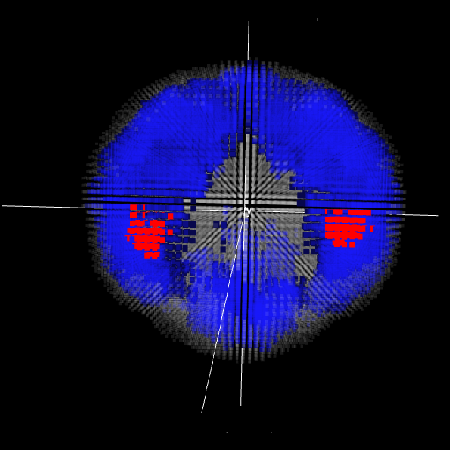
\includegraphics[width=.45\linewidth]{gfx/chapter2/cell1.png}} \quad
        \subfloat[X2C521L: Wnt8, HEN1-Y61, Gsx]
        {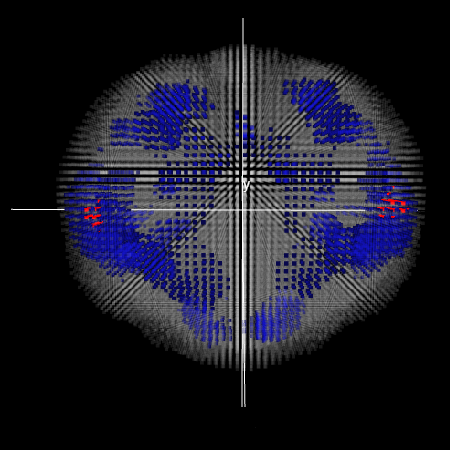
\includegraphics[width=.45\linewidth]{gfx/chapter2/cell2.png}} \\
        \subfloat[X2C61L: VAChT, ChaT, LYamide]
        {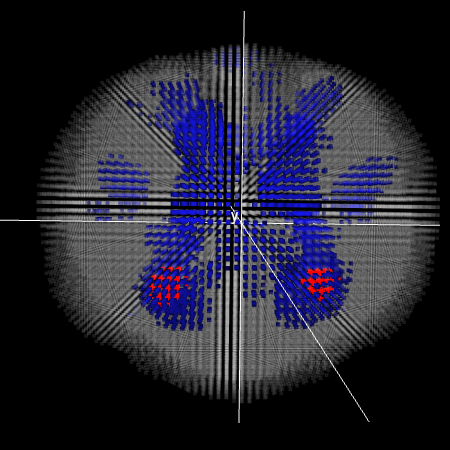
\includegraphics[width=.45\linewidth]{gfx/chapter2/cell3.png}} \quad
        \subfloat[X2C241S: Mitf, Otx, Tolloid-Y68]
        {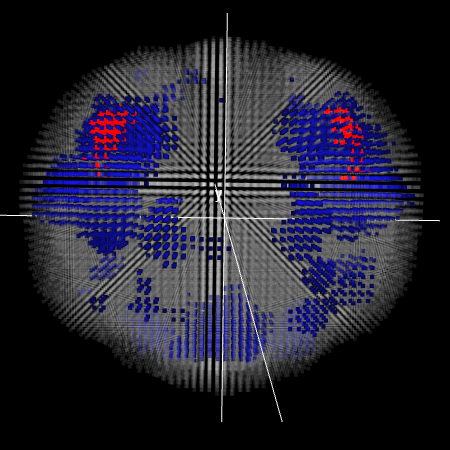
\includegraphics[width=.45\linewidth]{gfx/chapter2/cell4.png}}
        \caption{Regions defined by the expression overlap of the top 3 scoring genes in \citep{Tomer10} binarized in-situ hybridization data. The red colour shows the co-expression of the three considered genes, the blue areas are those where one or more of the three considrered genes are expressed but not all, in grey are the areas where none of the considered genes are expressed. The 4 figures are from a apical view with the dorsal side on top.}\label{fig:cell_localization}
\end{figure}

Overall, the results of this back-mapping method look very promising. Although at the time of writing, this work is still in progress in collaboration with Kaia Achim and Detlev Arendt, I have been able so far to map-back 27 of the 38 live single cells to a defined area of overlapping expression in the brain using the top 3 or 4 most specific genes. The cells were mapped to an average of 100 cubes defining a spatially coherent region. \\

I decided to check the probability of obtaining such a result by chance. To this end, I randomly generated 1000 ``top 3'' genes out of the 86 genes considered in the in-situ hybridization data. For each of these ``top 3'' randomly generated genes, I computed the number of cubes in the in-situ hybridization dataset where the 3 genes were co-expressed.\\

Subsequently, I compared the number of overlapping cubes obtained with this random process to the number of overlapping cubes obtained with the top 3 most specific genes from the 38 live single cells. The results are shown as boxplots in Figure \ref{fig:boxplot_rna}. The left hand part of the plot shows the number of cubes obtained with the genes selected randomly. In this case the mean number of cubes if extremely close to zero . The right hand part of the plot shows the same results for the top 3 most specifically expressed genes of the 38 alive cells in the single cell RNA-seq dataset and clearly shows an enrichment on the non randomized side. 

	\begin{figure}[H]
\centerline{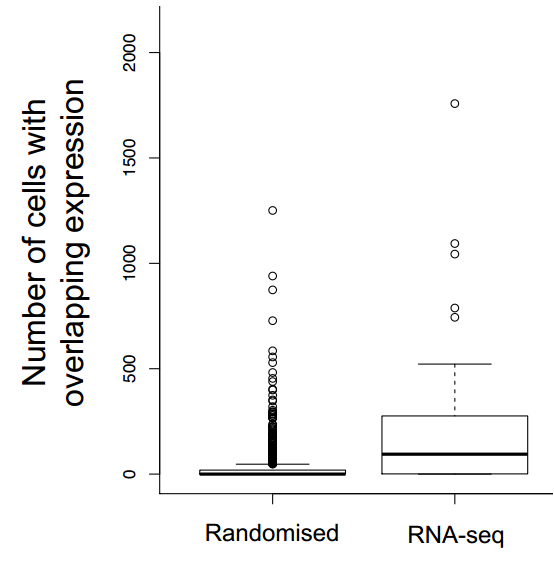
\includegraphics[width=0.6\linewidth]{gfx/chapter2/rand_top3.png}}
\caption{{\bf Back-mapping by chance vs RNA-seq data.} This boxplot shows the number of ``cubes'' in which the top 3 genes overlap with randomly generated top 3 genes (left N=1000) and the top 3 genes obtained from the live single cells RNA-seq data(N=38).}\label{fig:boxplot_rna}
	\end{figure}
	
  \subsection{Binarizing whole transcriptomes}
  
  Even though the back-mapping method describe previously manages to deal with the noise in the data by looking at the most specifically expressed genes, as mentioned for in-situ hybridization, for other methods it could be useful to binarize the data. When dealing with whole transcriptomes, manually finding thresholds to binarize gene expression data is no longer a valid option due to the high number of genes considered. An automated method is thus required. I will discuss possible ways to binarize single cell RNA-seq data, presenting some results cells from the brain of \platy{}.\\
  
  A naive approach would be to simply consider that as long as one RNA fragment mapped to a particular gene has been found in a cell, the gene is considered as expressed. Although such a method would be justifiable in the case of a perfect dataset, with no noise or errors, as discussed above \ref{sec:quantitative_single_cell} in the case of single cell RNA-seq the biases created by the mRNA capture rate are to high to rely simply on this method. Indeed, as a first approach on \platy{}'s dataset, we can see on Figure \ref{fig:hist_rna} that the value $0$ represents a very dominant peak. The problem in that case is that for read counts of $0$ it is dangerous to consider the gene as non expressed when it could be lowly expressed.\\
  
\begin{figure}[H]
        \myfloatalign
        \subfloat[Histogram showing the frequencies of count values over 72 sequenced cells, with the fragments mapped to 169 genes.]
        {\label{fig:hist_rna}
        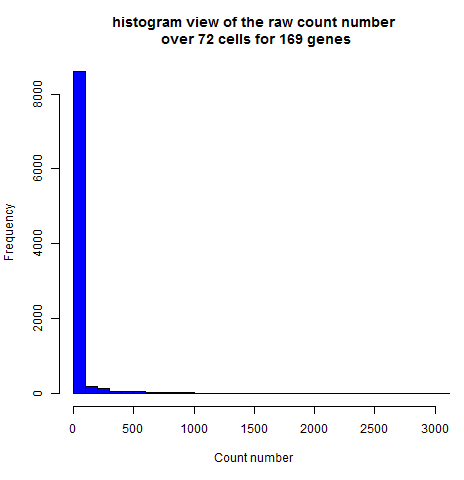
\includegraphics[width=.8\linewidth]{gfx/chapter2/hist_rna.png}} \\
        \subfloat[Density plot for the count values over $0$ in the single cell sequencing dataset]
        {\label{fig:density_rna}%
         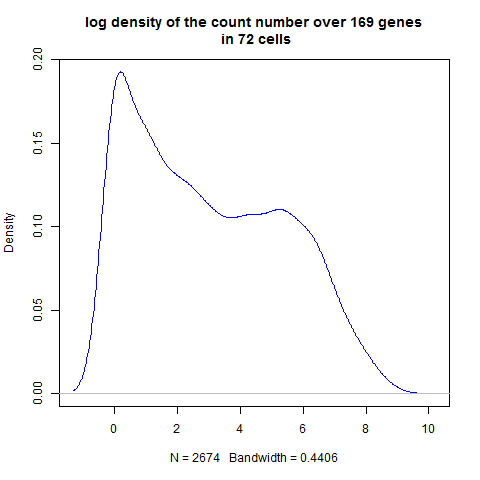
\includegraphics[width=.8\linewidth]{gfx/chapter2/density_rna.png}}
        \caption{Thresholding RNA sequencing data for \platy{}. The RNA-seq reads are mapped for the 72 cells to 169 genes in the PrimR dataset. This choice was made because at the moment the full genome of \platy{} is not available for mapping the reads. I believe however that mapping to the entire genome would improve the results significantly.}\label{fig:platynereis_single_cell}
\end{figure}
  
  Another option would be to find a global threshold over the complete dataset. The threshold, $T>0$, would represent the count number of reads for a particular gene and a particular cell needed to consider the gene as expressed. $T$ could be inferred from the count density over all the genes and all the cells. The expected result would be a 2 peak density with one peak corresponding to the non expressed count values, the second to expressed genes. The binary threshold would then be set between the first and second peak. Although more precise than the previous method, binarizing in such a manner may lead to numerous errors. Indeed, the underlying assumption behind this method is that all genes behave in a similar way. As Figure \ref{fig:density_rna} shows, if a 2 peak behaviour is indeed present, the cut is not extremely clear and an important portion of count numbers actually fall in between the two peaks. This is due to the fact that all expressed genes are not expressed in the same way; some are expressed lowly, some highly. As a result, the density curve tends to flatten making this thresholding method, if better, still not 100\% reliable.\\
  
  The more suitable approach to this thresholding problem would be to compute one threshold per gene based on the density curve for every gene across all cells. However, considering the sparse nature of the count data, no significant results can be extracted with this method without a large enough number of sequenced cells. However, I believe that one threshold per gene would result in a big improvement over the previously mentioned thresholding methods providing sufficient number of data points per gene.

